%------------------------------------------------------------------------
%Editar Diplomado
\hypertarget{cv:eliminarAccion}{\section{Eliminar Acción}} \label{sec:eliminarAccion}

	Esta funcionalidad le permitirá eliminar una acción innecesaria o incorrecta. Para eliminar la acción es necesario que no se encuentre asociada a casos de uso.
		\subsection{Procedimiento}

			%Pasos de procedimiento
			\begin{enumerate}
	
			\item Oprima el botón \IUBotonEliminar{} de un registro existente de la pantalla \ref{fig:GestionarAcciones} ''Gestionar Acciones''.
	
			\item Se mostrará el mensaje \ref{fig:confirmaEliminaAccion} sobre la pantalla \ref{fig:GestionarAcciones} ''Gestionar Acciones''.
			
			%Pantalla
			\begin{figure}[htbp!]
				\begin{center}
					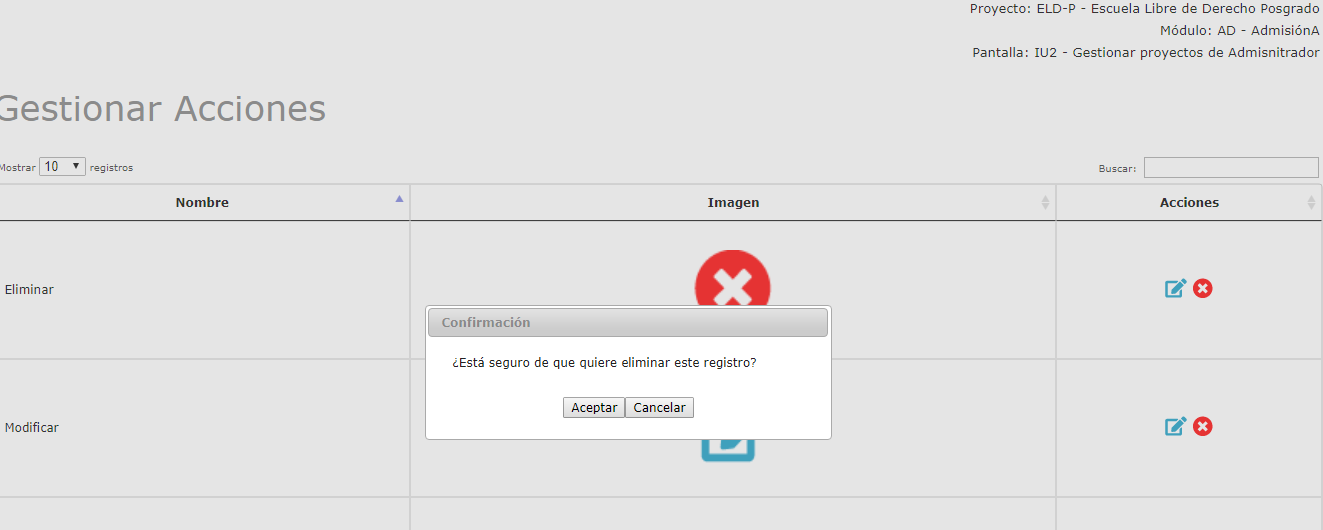
\includegraphics[scale=0.5]{roles/lider/pantallas/acciones/pantallas/IU11-1-1-3MSG10}
					\caption{MSG de Confirmación}
					\label{fig:confirmaEliminaAccion}
				\end{center}
			\end{figure}
						
			\item Oprima el botón \IUAceptar.
			
			\item Se mostrará el mensaje \ref{fig:accionEliminada} en la pantalla \ref{fig:GestionarAcciones} ''Gestionar Acciones''.
			
			\begin{figure}[htbp!]
				\begin{center}
					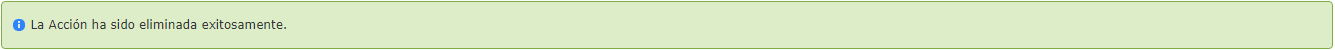
\includegraphics[scale=0.5]{roles/lider/pantallas/acciones/pantallas/IU11-1-1-3MSG1}
					\caption{MSG: Acción Eliminada}
					\label{fig:accionEliminada}
				\end{center}
			\end{figure}
			\end{enumerate}